\documentclass[9pt,fleqn,twoside,twocolumn]{stdglobal}

\fancypagestyle{sectionstyle}{
  \fancyhf{}
  \fancyhead[L]{\footnotesize\itshape Seminar (Theoretical Informatics Unplugged) 2021/2022}
  % \fancyfoot[C]{\footnotesize\bigskip\thepage/\pageref{LastPage}}
  % \fancyfoot{}
  \fancyfoot[C]{\footnotesize\bigskip\thepage}
  \fancyfoot[R]{\footnotesize\bigskip\copyright\ Markus Pawellek, \today}
  \renewcommand{\footrulewidth}{0.5pt}
  \renewcommand{\headrulewidth}{0pt}
}

\fancypagestyle{mainstyle}{
  \fancyhf{}
  \fancyfoot[C]{\footnotesize\bigskip\thepage}
  \fancyfoot[R]{\footnotesize\bigskip\copyright\ Markus Pawellek, \today}
  % \fancyhead[LO,RE]{\footnotesize \thetitle} %left
  % \fancyhead[RO,LE]{\footnotesize \theauthor} %right
  % \fancyhead[LO,RE]{\footnotesize \ \smallskip}
  \fancyhead[RO]{\footnotesize \@title \smallskip} %right
  \fancyhead[LE]{\footnotesize \@title \smallskip} %right
  \renewcommand{\headrulewidth}{0.5pt}
  \renewcommand{\footrulewidth}{0.5pt}
}

\usepackage{titlesec}
\titleformat{\section}{\normalfont\bfseries}{\thesection}{1em}{}

\title{%
  Probabilistic Circuits: Marginal Maximum a Posterioi Queries
}
%\subtitle{Seminar Report}
\author{Markus Pawellek}

\bibliography{references}

\DeclareMathOperator*{\argmax}{arg\ max}
\DeclareMathOperator{\val}{val}
\DeclareMathOperator{\nodein}{in}

\begin{document}

\selectlanguage{english}
\thispagestyle{sectionstyle}

\twocolumn[{\begin{@twocolumnfalse}%
  \begin{center}
    \Large
    \bfseries
    Probabilistic Circuits: \\
    Marginal Maximum a Posteriori Queries
  \end{center}%
  \begin{center}
    Markus Pawellek \\
    markus.pawellek@mailbox.org
  \end{center}
  \vspace{1em}
  \hrule
  \begin{abstract}
    \itshape
    \noindent
    Marginal maximum a posteriori (MMAP) queries combine the aspects of both marginal (MAR) and maximum a posteriori (MAP) inference.
    Introducing marginal determinism, we are able to provide sufficient conditions for a probabilistic circuit (PC) to be tractable for these queries.
    % By replacing the given PC with its respective sum-maximizer circuit, MMAP queries can be computed with a simple feed-forward traversal.
    To handle MMAP queries in this case, the computation of sum units based on the algorithms for MAR and MAP queries is adjusted.
  \end{abstract}
  \hrule
  \vspace{1.5em}
\end{@twocolumnfalse}}]


\section{Introduction}
  This report is a summary of the tractable computation of marginal maximum a posteriori (MMAP) queries for probabilistic circuits (PCs) based on the sections 8.1 and 8.2 of the article \citetitle{pc-framework} by \textcite{pc-framework}.
  To facilitate notation, no boldface variables are used.

\section{Background}
  For the scope of this report, we define the following.
  \[
    \begin{aligned}[t]
      X &\ldots \text{finite set of random variables} \\
      p\, &\ldots \text{joint probability distribution over $X$} \\
      \mathscr{C}\, &\ldots \text{PC over $X$ with $\mathscr{C}=(\mathscr{G},ϑ)$} \\
      Q &\ldots \text{set of query variables with $Q\subset X$}
    \end{aligned}
  \]
  \begin{definition*}[(MMAP Query Class)]
    Define $\mathscr{Q}_\mathrm{MMAP}(Q)$ as the set of MMAP queries over $Q$ such that the following holds.
    % For all sets $E$ and $Z$, that form a partition of $X\setminus Q$, for all $e\in E$ and intervals $\mathscr{I}\subset \val(Z)$, it contains a query that computes the following expression.
    % The elements of the class $\mathscr{Q}_\mathrm{MMAP}(Q)$ of MMAP queries over $Q$ compute the following expression for all sets of evidence variables $E$ and marginal variables $Z$, that form a partition of $X\setminus Q$, and partial states $e\in E$ and sets of intervals $\mathscr{I}\subset\val(Z)$ to be marginalized over.
    \[
      \begin{aligned}
        &\forall\ \text{partitions } \set{E,Z}{} \text{ of } X\setminus Q: \\
        &\forall\ e\in E \text{ and intervals } \mathscr{I}\subset\val(Z): \\
        &\exists\ \mathscr{A}\in \mathscr{Q}_\mathrm{MMAP}(Q):\quad \mathscr{A} \text{ computes } \\
      \end{aligned}
    \]
    \[
      \quad\argmax_{q\in \val(Q)}\ p\roundBrackets{Q = q \ |\ E = e, Z\in \mathscr{I}}
    \]
    % Hereby, $E$ may be called the set of evidence variables, $Z$ the set of marginal variables, $e$ the partial state, and $I$ marginalization interval.
  \end{definition*}
  % \noindent
  Because maximization is not affected by normalization constants, we can also use the following equivalent expression for the above definition.
  \[
    \argmax_{q\in \val(Q)} \integral{\mathscr{I}}{}{p(q,e,z)}{Z}
  \]

  % As a direct consequence, we see, by setting $\mathbf{Q}=\emptyset$ or $\mathbf{Q}=\mathbf{X}$, that the MMAP query class subsumes both MAR and MAP queries.
  \noindent
  As a result, the connection to marginal (MAR) and maximum a posteriori (MAP) queries can be seen.
  \[
    \begin{aligned}[t]
      &\mathbf{case}\ Q=\emptyset\ : &\mathscr{Q}_\mathrm{MMAP}(Q) &= \mathscr{Q}_\mathrm{MAR} \\
      &\mathbf{case}\ Q=X: &\mathscr{Q}_\mathrm{MMAP}(Q) &\subset \mathscr{Q}_\mathrm{MAP}
    \end{aligned}
  \]
  Now, recapitulate the characterizing properties for a PC to be tractable for those queries.
  \[
    \begin{aligned}[t]
      &\text{$\mathscr{C}$ is tractable for MAR queries} \\
      &\iff \text{$\mathscr{G}$ is decomposable and smooth}
    \end{aligned}
  \]
  \[
    \begin{aligned}[t]
      &\text{$\mathscr{C}$ is tractable for MAP queries} \\
      &\iff \text{$\mathscr{G}$ is consistent and deterministic}
    \end{aligned}
  \]
  \[
    \text{$\mathscr{G}$ is decomposable} \implies \text{$\mathscr{G}$ is consistent}
  \]
  % Please recapitulate that for a PC, the ability to tractably compute MAR queries is equivalent to its smoothness and decomposability.
  % The tractable computation of MAP queries in a PC is characterized by the properties consistency and determinism.
  % Also, decomposability implies consistency.
  % Hence, a smooth, decomposable, and deterministic PC is able tractably compute MAP and MAR queries.
  % As a consequence, we will assume a given PC should be smooth and decomposable.
  % As a consequence, we need a property that generalizes determinism to a weaker property.


  % Marginal (MAR) queries in the following sense are of paramount importance when we want to reason about state of the world where not all random variables are fully observed.
  % \[
  %   p(E=e, Z\in I) = \integral{I}{}{p(z,e)}{Z}
  % \]

  % Maximum a posteriori (MAP) queries relate to the mode of the distribution in the following sense.
  % \[
  %   \argmax_{q\in\val(Q)} p(q\ |\ e) = \argmax_{q\in\val(Q)} p(q, e)
  % \]


\section{Tractable Computations of MMAP Queries}
  \begin{definition*}[(Marginal Determinism)]
    A sum node $n\in\mathscr{G}$ with inputs $r_c$ for $c\in\nodein(n)$ is $Q$-marginal deterministic if
    \begin{align*}
      \forall q\in\val(Q):
      &\ \forall c\in\nodein(n): r_c = 0 \\
      &\vee\ \exists! c\in\nodein(n): r_c \neq 0
    \end{align*}
    % A sum node is marginal deterministic with respect to $\mathbf{Q}$ if for any partial state $\mathbf{q}\in\val(\mathbf{Q})$, the output of at most one of its input units is nonzero.
    If this holds for all sum nodes $n\in\mathscr{G}$ with $φ(n)\cap Q\neq\emptyset$, also $\mathscr{G}$ is called $Q$-marginal deterministic.
    % $\mathscr{G}$ is $Q$-marginal deterministic if all of its sum nodes containing variables of $\mathbf{Q}$ in its scope are $Q$-marginal deterministic.
  \end{definition*}
  \vspace{-0.1em}
  \noindent
  % Because decomposability implies consistency, we will restrict ourselves to smooth and decomposable PCs.
  Marginal determinism is a simple generalization of determinism.
  Based on this definition, it now becomes clear, how to use the MAP and MAR algorithms to tractably compute MMAP queries given $\mathscr{G}$ being smooth, decomposable, and $Q$-marginal deterministic.

  As always, we assume that an input unit already computes the given query correctly.
  Concerning the output of product units, the computations for MAR and MAP queries are identical and only involve the multiplication of their inputs.
  As a result, product units shall be treated the same way for this algorithm.
  For sum units on the other hand, a decision has to be made based on whether their scope intersects with $Q$.

  Let $n\in\mathscr{G}$ be a sum unit with output $r_n$, inputs $r_c$, and  weights $ϑ_{nc}$ for $c\in\nodein(n)$ in a feed-forward traversal of $\mathscr{C}$.
  Then its result $r_n$ can be computed by the following snippet.
  \medskip
  \begin{tcolorbox}[%
    colframe=black,
    colbacktitle=white,
    coltitle=black,
    colback=mathdefback,
    attach boxed title to top center={yshift=-2mm},
    enhanced,
    titlerule=0.1pt,
    boxrule=0.5pt,
    arc=5pt,
    breakable,
    title=Sum Unit Computation for MMAP Algorithm
  ]
    \vspace{-1em}
    \[
      \begin{aligned}[t]
        \mathbf{if}\quad &φ(n) \cap Q \neq \emptyset \quad \mathbf{then} \\
        & r_n \longleftarrow \max_{c\in\nodein(n)} ϑ_{nc}r_c \\
        \mathbf{else} \\
        & r_n \longleftarrow \sum_{c\in\nodein(n)} ϑ_{nc}r_c
      \end{aligned}
    \]
  \end{tcolorbox}

  \noindent
  Remember from the MAP algorithm, that at the end of the whole algorithm a backward pass is needed to retrieve the modes of the input distributions that contributed to the output.

  \begin{theorem*}[(Sufficient Conditions)]
    Let $\mathscr{G}$ be smooth, decomposable, and $Q$-marginal deterministic.
    Then for any parameterization $ϑ$ the above algorithm
    % the sum-maximizer circuit of $\mathscr{G}$
    tractably computes MMAP queries of $\mathscr{C}$ over $Q$.
  \end{theorem*}
  \begin{proof}
    Let $E$ and $Z$ be a partition of $X\setminus Q$.
    Furthermore, let $e\in E$ be a partial state, $\mathscr{I}\in\val(Z)$ an interval, and $\mathscr{Q}(e,\mathscr{I})$ be the MMAP query.
    Then the statement is proved by induction.
    \[
      \mathscr{Q}(e,\mathscr{I}) = \max_{q\in\val(Q)} \integral{\mathscr{I}}{}{\mathscr{C}(Z,q,e)}{Z}
    \]

    The root node $n\in\mathscr{G}$ can be one of three types: input unit, sum unit, or product unit.
    By definition, input units already output the correct values for $\mathscr{Q}(e,\mathscr{I})$.

    Due to decomposability, for product units, we are allowed to assume that $Z$, $Q$, and $E$ are partitioned into $Z_i$, $Q_i$, and $E_i$ for $i,k\in\setNatural$ and $i\leq k$, respectively.
    \begin{align*}
      \mathscr{Q}(e,\mathscr{I}) &= \max_{q_1,\ldots,q_k\in\val(Q)} \integral{\mathscr{I}}{}{\prod_{i=1}^k\mathscr{C}_i(Z_i,q_i,e_i)}{Z} \\
      &= \max_{q_1,\ldots,q_k\in\val(Q)} \prod_{i=1}^k \integral{\mathscr{I}}{}{\mathscr{C}_i(Z_i,q_i,e_i)}{Z_i} \\
      &= \prod_{i=1}^k \max_{q_i\in\val(Q)} \integral{\mathscr{I}_i}{}{\mathscr{C}_i(Z_i,q_i,e_i)}{Z_i} \\
      &= \prod_{i=1}^k \mathscr{Q}_i(e_i,\mathscr{I}_i)
    \end{align*}

    Sum units, whose scope contains no query variable, only compute MAR queries.
    Their correct behavior was already proven.
    So, assume $n$ to be a sum unit with $φ(n)\cap Q \neq \emptyset$.
    \begin{align*}
      \mathscr{Q}(e,\mathscr{I}) &= \max_{q\in\val(Q)} \integral{\mathscr{I}}{}{\sum_{i\in\nodein(n)} ϑ_i\mathscr{C}_i(Z,q,e)}{Z} \\
      &= \max_{q\in\val(Q)} \sum_{i\in\nodein(n)} \integral{\mathscr{I}}{}{ϑ_i\mathscr{C}_i(Z,q,e)}{Z} \\
      &= \max_{q\in\val(Q)} \max_{i\in\nodein(n)} \integral{\mathscr{I}}{}{ϑ_i\mathscr{C}_i(Z,q,e)}{Z} \\
      &= \max_{i\in\nodein(n)} ϑ_i \max_{q\in\val(Q)} \integral{\mathscr{I}}{}{\mathscr{C}_i(Z,q,e)}{Z} \\
      &= \max_{i\in\nodein(n)} ϑ_i \mathscr{Q}_i(e,\mathscr{I})
    \end{align*}
    For this, smoothness and $Q$-marginal determinism has been used.
    Applying these equations recursively down to input units, this concludes the proof.
  \end{proof}

% \section{Example}
%   \begin{figure}[H]
%     \center
%     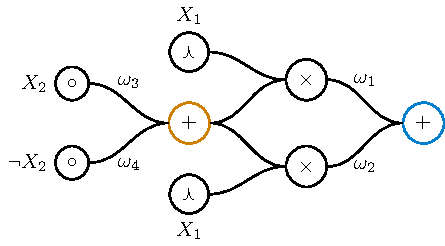
\includegraphics[width=0.45\textwidth]{figures/example.pdf}
%   \end{figure}
%   \begin{align*}
%     \mathscr{C}(x_1,x_2)
%     = &\boxBrackets{ ω_1f_1(x_1) + ω_2f_2(x_1)} \\
%     &\times \boxBrackets{ ω_3 x_2 + ω_4 (1-x_2) }
%   \end{align*}
%   \begin{align*}
%     &\max_{x_2\in\set{0,1}{}} \integral{}{}{\mathscr{C}(x_1,x_2)}{X_1}
%     = \max\set{ω_3,ω_4}{} \times \\
%     &\boxBrackets{ ω_1 \integral{}{}{f_1(x_1)}{X_1} + ω_2 \integral{}{}{f_2(x_1)}{X_1}}
%   \end{align*}

\section{Conclusions}
  The computation complexity of the set of marginal MMAP queries may typically be NP-hard and is highly dependent on the set of query variables.
  For examining the efficient evaluation of MMAP queries for PCs, the structural property of marginal determinism was defined.
  Together with smoothness and decomposability, these are sufficient conditions to make PCs tractable for MMAP queries.
  Nevertheless, using the more general structure of sum-maximizer circuits, it can be shown that these properties are indeed not necessary.
  %For the extreme case of the query set, the MMAP query collapses to either a marginal (MAR) or a maximum a posteriori (MAP) query.
  %As a consequence, also the tractable computation of other query types, such as marginal entropy or mutual information, is made possible.

  As an outlook: In contrast to other structural properties, marginal determinism was defined with respect to its query set.
  % For $Q=\emptyset$, it corresponds to smooth and decomposable PCs (tractable for MAR).
  % For $Q=X$, it corresponds to smooth, decomposable, and deterministic PCs (tractable for both MAR and MAP).
  % The latter is more expressive efficient.
  % Other subsets may not be as expressive efficient with respect to either a subset or a superset.
  Assuming marginal determinism for all possible subsets of $X$, $\mathscr{C}$ cannot contain a full-support distribution without it to be fully factorized.
  The family of such PCs thus is not expressive and would therefore impose a too strong restriction.

\nocite{*}
\AtNextBibliography{\footnotesize}
\printbibliography[heading=bibintoc]

\end{document}
